%!TEX root = ../thesis.tex
% ******************************* Thesis Appendix E ********************************

\chapter{GEANT4 Light Output Vs. Fitted Light Output}

\begin{figure}[htbp]
\centering
\begin{subfigure}{.49\textwidth}
  \centering
  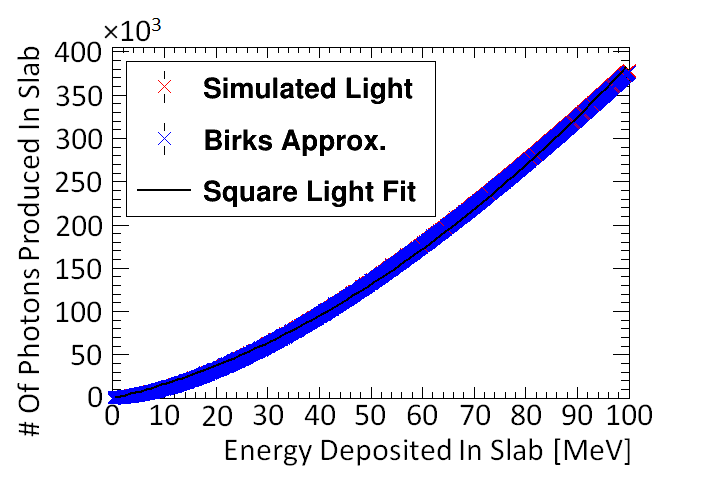
\includegraphics[width=\linewidth]{Appendix5/newNewFigs/alphaBirksSlab_simAndApproxLight.png}
  \captionsetup{width=.9\linewidth}
  \caption{}
  \label{subfig:append5_light_of_Alphas0-100mev}
\end{subfigure}
\begin{subfigure}{.49\textwidth}
  \centering
  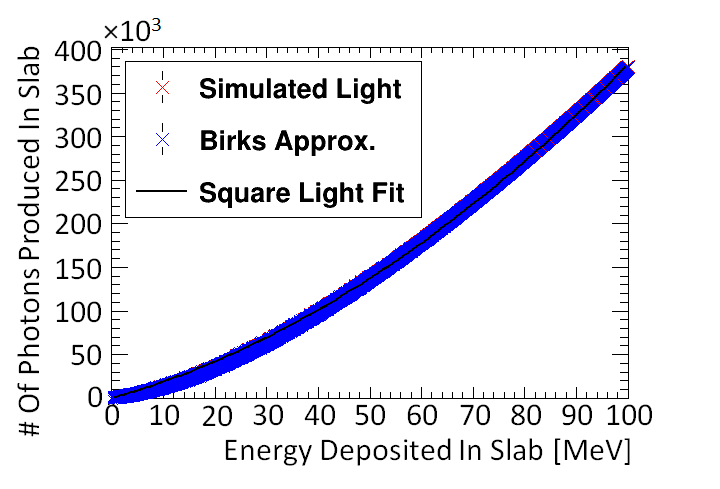
\includegraphics[width=\linewidth]{Appendix5/newNewFigs/aAlphaBirksSlab_simAndApproxLight.png}
  \captionsetup{width=.9\linewidth}
  \caption{}
  \label{subfig:append5_light_of_AAlphas0-100mev}
\end{subfigure}
\caption[Birks' light approximation for alpha particles compared to simulation.]{How the Birks approximation (equation \ref{equ:Birks_formula}) approximates light for 1E6 alpha particles in (a) and 1E6 anti-alpha particles in (b). The Birks approximation is very suitable for these particles.}
\label{fig:append5_light_of_Alphas_AAlphas0-100mev}
\end{figure}

\begin{figure}[htbp]
\centering
\begin{subfigure}{.5\textwidth}
  \centering
  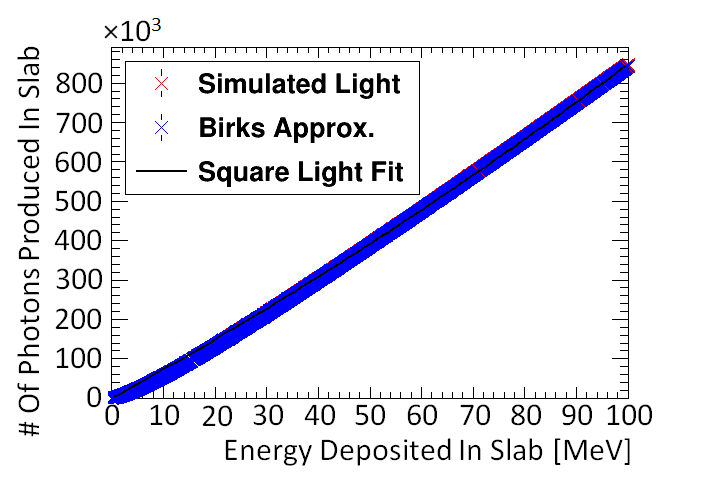
\includegraphics[width=\linewidth]{Appendix5/newNewFigs/protonBirksSlab_simAndApproxLight.png}
  \captionsetup{width=.9\linewidth}
  \caption{}
  \label{subfig:append5_light_of_protons0-100mev}
\end{subfigure}%
\begin{subfigure}{.5\textwidth}
  \centering
  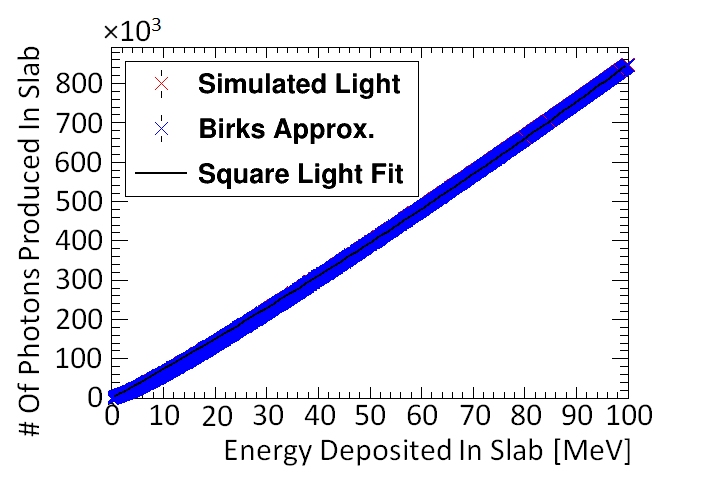
\includegraphics[width=\linewidth]{Appendix5/newNewFigs/aProtonBirksSlab_simAndApproxLight.png}
  \captionsetup{width=.9\linewidth}
  \caption{}
  \label{subfig:append5_light_of_Aprotons0-100mev}
\end{subfigure}
\caption[Birks' light approximation for proton particles compared to simulation.]{How the Birks approximation (equation \ref{equ:Birks_formula}) approximates light for 1E6 protons in (a) and 1E6 anti-protons in (b). The Birks approximation is very suitable for these particles.}
\label{fig:append5_light_of_protons_Aprotons0-100mev}
\end{figure}

\begin{figure}[htbp]
\centering
\begin{subfigure}{.5\textwidth}
  \centering
  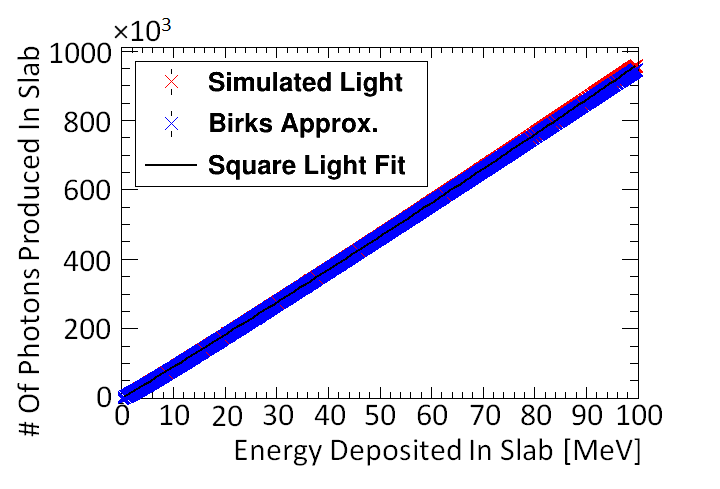
\includegraphics[width=\linewidth]{Appendix5/newNewFigs/pi+BirksSlab_simAndApproxLight.png}
  \captionsetup{width=.9\linewidth}
  \caption{}
  \label{subfig:append5_light_of_pIPlus0-100mev}
\end{subfigure}%
\begin{subfigure}{.5\textwidth}
  \centering
  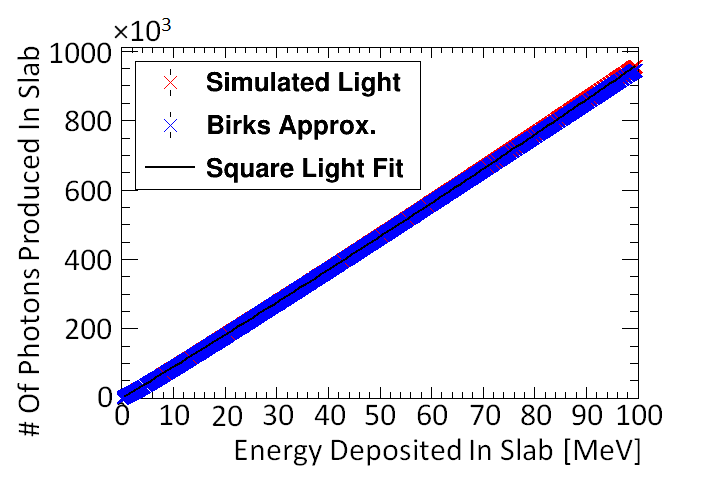
\includegraphics[width=\linewidth]{Appendix5/newNewFigs/pi-BirksSlab_simAndApproxLight.png}
  \captionsetup{width=.9\linewidth}
  \caption{}
  \label{subfig:append5_light_of_pIMinus0-100mev}
\end{subfigure}
\caption[Birks' light approximation for pion particles compared to simulation.]{How the Birks approximation (equation \ref{equ:Birks_formula}) approximates light for 1E6 positive pions in (a) and 1E6 negative pions in (b).}
\label{fig:append5_light_of_pIPlus_pIMinus0-100mev}
\end{figure}

\begin{figure}[htbp]
\centering
\begin{subfigure}{.5\textwidth}
  \centering
  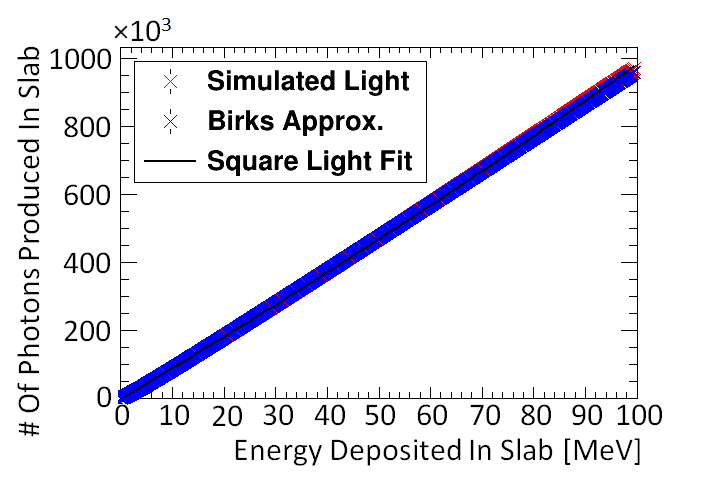
\includegraphics[width=\linewidth]{Appendix5/newNewFigs/mu-BirksSlab_simAndApproxLight.png}
  \captionsetup{width=.9\linewidth}
  \caption{}
  \label{subfig:append5_light_of_muons0-100mev}
\end{subfigure}%
\begin{subfigure}{.5\textwidth}
  \centering
  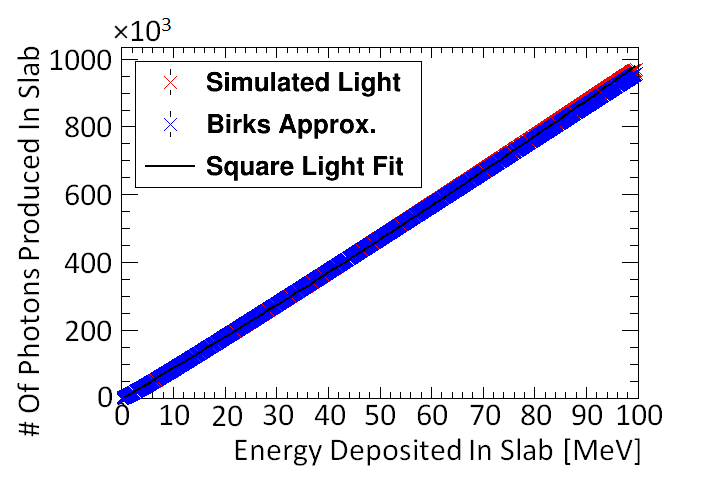
\includegraphics[width=\linewidth]{Appendix5/newNewFigs/mu+BirksSlab_simAndApproxLight.png}
  \captionsetup{width=.9\linewidth}
  \caption{}
  \label{subfig:append5_light_of_Amuons0-100mev}
\end{subfigure}
\caption[Birks' light approximation for muon particles compared to simulation.]{How the Birks approximation (equation \ref{equ:Birks_formula}) approximates light for 1E6 muons in (a) and 1E6 anti-muons 1E6 in (b). The Birks approximation is very suitable for these particles.}
\label{fig:append5_light_of_muons_Amuons0-100mev}
\end{figure}

\begin{figure}[htbp]
\centering
\begin{subfigure}{.5\textwidth}
  \centering
  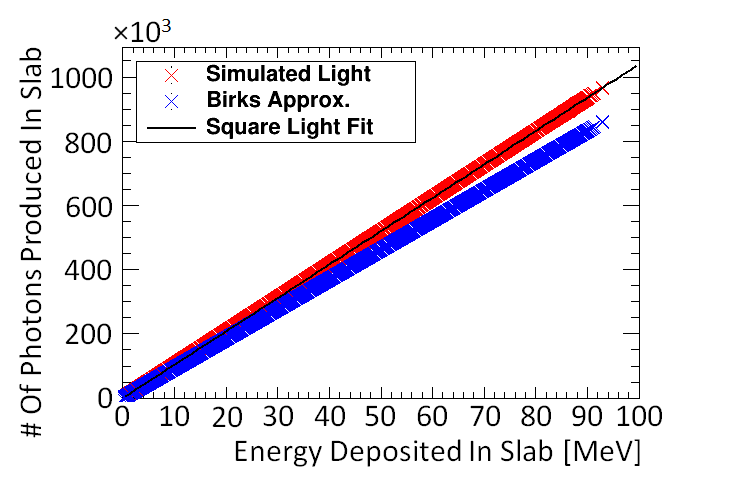
\includegraphics[width=\linewidth]{Chapter4/Figs/Raster/electronSimulatedLightNew.png}
  \captionsetup{width=.9\linewidth}
  \caption{}
  \label{subfig:append5_light_of_electrons0-100mev}
\end{subfigure}%
\begin{subfigure}{.5\textwidth}
  \centering
  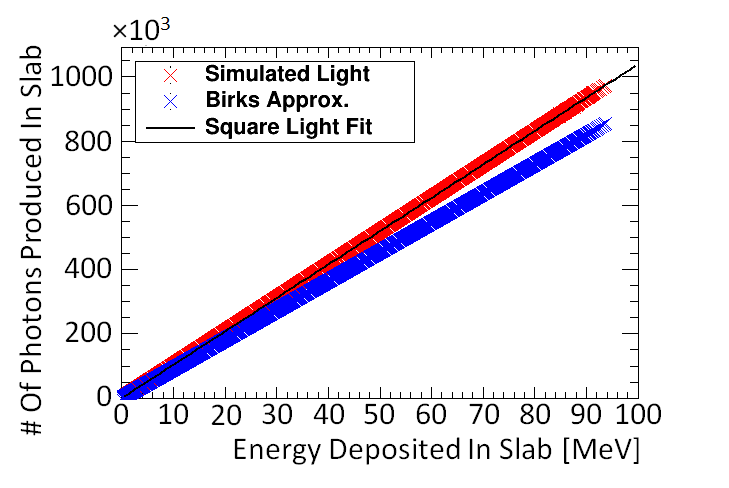
\includegraphics[width=\linewidth]{Chapter4/Figs/Raster/positronSimulatedLightNew.png}
  \captionsetup{width=.9\linewidth}
  \caption{}
  \label{subfig:append5_light_of_positrons0-100mev}
\end{subfigure}
\caption[Birks' light approximation for electrons and positrons compared to simulation.]{How the Birks approximation (equation \ref{equ:Birks_formula}) approximates light for 1E6 electrons in (a) and 1E6 positrons in (b). The Birks approximation is alone is unsuitable.}
\label{fig:append5_light_of_electrons_positrons0-100mev}
\end{figure}

\begin{figure}[htbp]
\centering
\begin{subfigure}{.5\textwidth}
  \centering
  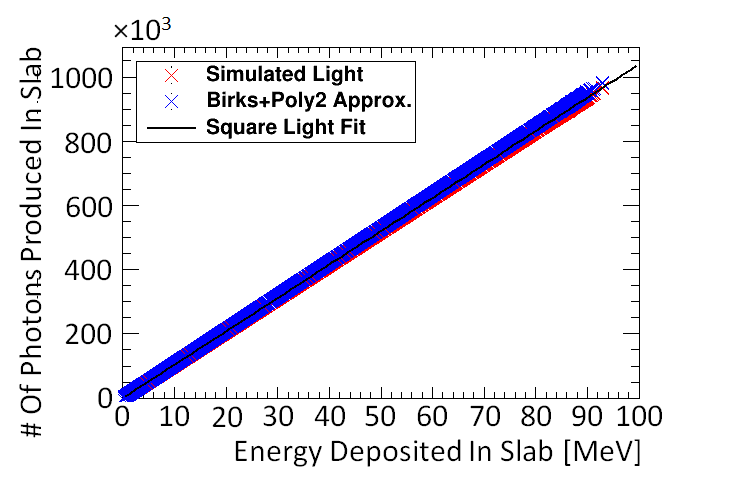
\includegraphics[width=\linewidth]{Chapter4/Figs/Raster/electronSimulatedLightBirksAndPoly2New.png}
  \captionsetup{width=.9\linewidth}
  \caption{}
  \label{subfig:append5_light_of_electronsLin0-100mev}
\end{subfigure}%
\begin{subfigure}{.5\textwidth}
  \centering
  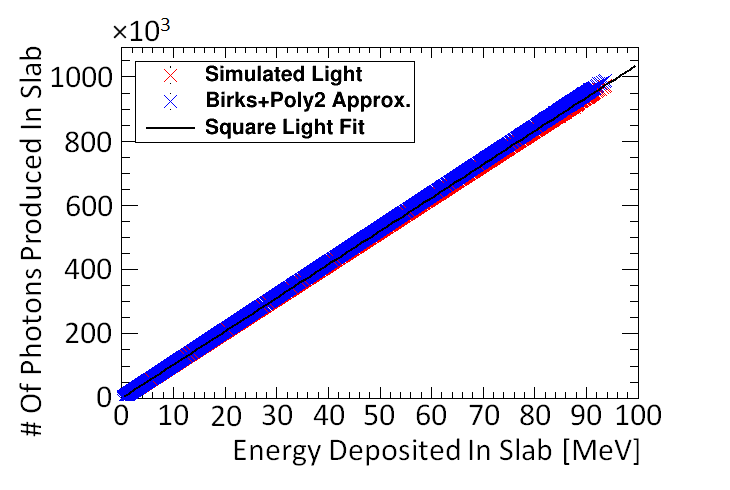
\includegraphics[width=\linewidth]{Chapter4/Figs/Raster/positronSimulatedLightBirksAndPoly2New.png}
  \captionsetup{width=.9\linewidth}
  \caption{}
  \label{subfig:append5_light_of_positronsLin0-100mev}
\end{subfigure}
\caption[Birks' light approximation + 2$^\textrm{nd}$ order polynomial for electrons and positrons compared to simulation.]{The simulated light for 1E6 electrons in (a) and 1E6 positrons particles in (b). The approximation for $dE/dx$ is a combination of the Birks law for high values of $dE/dx$ (2 and above) and a polynomial 2 fit between 0-2. Thus approximating the light successfully.}
\label{fig:append5_light_of_electrons_positronsLin0-100mev}
\end{figure}